\documentclass[12pt,a4paper,twoside]{scrartcl}

\usepackage[utf8]{inputenc}
\usepackage[T1]{fontenc}
\usepackage{amsmath,amssymb,amsthm}
\usepackage{libertine}
\usepackage{fourier}
\usepackage{graphicx}

\setlength{\voffset}{-28.4mm}
\setlength{\hoffset}{-1in}
\setlength{\topmargin}{20mm}
\setlength{\oddsidemargin}{25mm}
\setlength{\evensidemargin}{25mm}
\setlength{\textwidth}{160mm}

\setlength{\parindent}{0pt}

\setlength{\textheight}{235mm}
\setlength{\footskip}{20mm}
\setlength{\headsep}{50pt}
\setlength{\headheight}{0pt} 

\newcommand\var[1]{{\operatorname{#1}}}
% \var{eval}
% \var{span}
% \var{Hom}
% \var{Der}
% Composition = .
% \delta_{i,j} Kronecher delta
\newcommand\Z[1]{\nicefrac{\integers}{#1\integers}}

%% General things
%       
        \newcommand\mkset[2]{\left\lbrace#1\,|\, #2\right\rbrace}
        \DeclareMathOperator\diag{\text{diag}}

% Number Sets
%
        \DeclareMathOperator\naturals{\mathbb N_0}
        \DeclareMathOperator\posnats{\mathbb N_{>0}}
        \DeclareMathOperator\integers{\mathbb Z}
        \DeclareMathOperator\rationals{\mathbb Q}
        \DeclareMathOperator\reals{\mathbb R}
        \DeclareMathOperator\complex{\mathbb C}

% Definitional Equality
%
        \DeclareMathOperator\defeq{\overset{\text{def}}=}


% Standard Varieties and related constructions
%
        \DeclareMathOperator\proj{\mathbb P}
        % projective variety for some ideal
        \DeclareMathOperator\V{\mathcal V}
        \DeclareMathOperator\I{\mathcal I}


% Morphism Arrows
%
        \newcommand\hookr\hookrightarrow  
        \newcommand\hookl\hookleftarrow  

%% Polynomial things
%
        \DeclareMathOperator\del\partial



\newtheorem{dummy}{dummy}[section]
\newtheorem{proposition}[dummy]{Proposition}
\newtheorem{corollary}[dummy]{Corollary}
\newtheorem{theorem}[dummy]{Theorem}
\newtheorem{lemma}[dummy]{Lemma}

\theoremstyle{definition}
\newtheorem{definition}[dummy]{Definition}

\theoremstyle{remark}
\newtheorem{example}[dummy]{Example}
\newtheorem{remark}[dummy]{Remark}


\newenvironment{todo}{
  \begin{framed}
  \textbf{TODO}
  \begin{itemize}
}{
  \end{itemize}
  \end{framed}
}



\title{Bachelor thesis: The 27 lines on the cubic}
\author{Long Huynh Huu}
\date{\today}

\begin{document}

\begin{titlepage}
\begin{center}

\includegraphics{TUMlschwarz.png}\\[3mm]
\sf
{\Large
  Technische Universit\"at M\"unchen\\[5mm]
  Department of Mathematics\\[8mm]
}
\normalsize
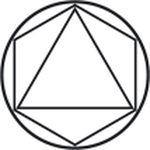
\includegraphics{TUMlMschwarz.png}\\[15mm]

Bachelor's Thesis\\[15mm]

{\Huge
  The 27 Lines on a Cubic Surface
}
\bigskip

\normalsize

Long Huynh Huu <long.huynh-huu@tum.de>
\end{center}
\vspace*{75mm}

Supervisor: Christian Liedtke <liedtke@ma.tum.de>
\medskip

Advisor: Christian Liedtke <liedtke@ma.tum.de>
\medskip

Submission Date: October 27th, 2014

\end{titlepage}

%%%% The following has to be signed by hand!

\vspace*{150mm}

I assure the single handed composition of this bachelor's thesis only supported by declared resources.
\bigskip

Garching, 
\newpage


\section*{Zusammenfassung}
%TODO: Auf Deutsch
xxxxxxxxxxxx deutsche Zusammenfassung xxxxxxxxxx

In this Bachelor thesis I will prove in full detail the existence of 27 lines on an arbitrary smooth cubic in projective $n$-space over an algebraically closed field $k$.

\newpage
\tableofcontents
\newpage

\pagenumbering{arabic}
\pagestyle{headings}


% \section{Change of coordinates}

\subsection{Notes to myself}

In this section I introduce definitions and hands-on examples to work with geometric objects in the language of scheme theory, or maybe I'll just drop the generalities and work with elementary algebra.
Particular goals are
\begin{itemize}
\item the definition of what a change of coordinates means precisely and work out the details to use it without regret in the proof of the main result.
\item the definition of what it means for a variety to contain a doubled line. In scheme theoretic language it is as simple as saying, that this variety has a subscheme isomorphic to a doubled line! Again, I might drop the notion of schemes, or work with it.
\end{itemize}
So this text also aims to be educational and close the gap between the intuitive and the technical.

It might be interesting to
\begin{itemize}
\item introduce the category of varieties and rational functions. \textbf{If needed}.
\end{itemize}

\subsection{Affine linear transformations of affine space}

An important notion which will appear again and again is the change of coordinates.
In affine space one thinks of a linear transformation $T:\affine^n_k \to \affine^n_k$.
Now observe the effect of such a transformation on a hypersurface $V(I)$, $I = (f)$:
$ T(V(I)) = \{ Tx \in k^n: f(x) = 0 \} = \{y \in k^n : f(T^{-1}y) = 0\}$
So one may define a linear transformation on a variety by precomposing the inverse to the polynomial functions.
But let me suggest a different definition of linear transformation which does not necessarily require $T$ to be invertible and which is compatible with the scheme theoretic notion of a morphism.

\begin{definition} Let $A = (a_{ij}) \in M(n,k)$ be a $n\times n$-matrix. Then we can define a homomorphism of polynomial rings
\begin{align}
T^\#_A : k[X_1,.. X_n] &\to k[X_1,.. X_n], \\
X_i &\to \sum_{j=1}^n a_{ij}X_j.
\end{align}
\end{definition}

This induces a morphism $T_A : \affine^n_k \to \affine^n_k$ of affine schemes. Indeed, this definition does what we expect.

\begin{proposition} By Hilbert's Nullstellensatz a point $(x_1,..x_n) \in k^n$ corresponds to a maximal ideal $(X_1-x_1,.. X_n-x_n) \subset k[X_1,..X_n]$.
$T_A$ maps the subscheme $V(X_1-x_1,..X_n-x_n)$ to $V(X_1-y_1,..X_n-y_n)$ where $(y_1,..y_n) = A(x_1,..x_n)$.
\end{proposition}

\begin{proof} If $A$ is invertible, we basically apply the Gauß-Jordan algorithm....
\end{proof}

Don't forget the translations: $X_i \mapsto X_i + t_i$.
Together we get affine linear transformations.


\subsection{Rational maps}

Fancy category language here...

\section{The twenty-seven lines}

After having proved all the basic geometric facts, we will turn our attention to finally prove the main theorem (for $\var{char}(k) \neq 2$).
\begin{theorem}
Let $k$ be an algebraically closed field, $\var{char } k \neq 2$ and let $S = \V(f) \subset \proj^3_k$ be a nonsingular cubic surface, $f\in k[x,y,z,t]$.
Then $S$ contains precisely 27 lines.
\end{theorem}
We will follow the proof given by Miles Reid (\cite[§7]{reid1988undergraduate}).

\subsection{Existence of a line}

We take an arbitrary point $P_0 \in S$ and consider its tangent plane $T_{P_0}(S) = \V(f^{(1)}(P_0))$.
Of course, no plane lies in $S$ completely, as this would imply the existence of singular points by Lemma \ref{lemmaSingularIntersect}.
By restricting the equation of $S$ to the tangent plane we obtain a 3-form $f' = f - f^{(1)}(P_0)g$, $g$ being some quadratic form.
If we're lucky $f'$ is reducible and hence a product of a linear and a quadratic form meaning that the intersection $T_{P_0}(S) \cap \V(f^{(1)}(R)) \simeq \V(f') \subset \proj^2_k$ is a union of a line and a conic (possibly a degenerate one).
So in this case $S$ contains a line.
Let's proceed assuming that we are unlucky and say $\V(f') \subset \proj^2_k$ is an irreducible cubic curve.
To simplify things, move tangent plane at $P_0$ to the plane $\V(t)$ and simultaneously move the point $P_0$ to $[0:0:1:0]$ by Corollary \ref{corollaryTransformPlaneWithPointOnIt}.
That this transforms the surface in a compatible manner with the tangent plane has been proven in proposition \ref{propositionTangentTransform}.
Eliminating the variable $t = 0$, $f(x,y,z,0)$ defines a cubic curve.
By Lemma \ref{lemmaIntersectionWithTangent} it is singular at $[0:0:1:0]$ and we know it is projectively equivalent to either $\V(x^2z - y^3)$ or $\V(x^3 + y^3 - xyz)$ by propositions \ref{propositionClassificationOfSingularCubics}, \ref{propositionNormalformCuspidal} and \ref{propositionNormalformNodal2}.
This however is only true if the characteristic of $k$ is not $3$, so we have to hope that the nodal case occurs somewhere.
We can lift this automorphism of the hyperplane $\V(t)$ to an automorphism of the whole space via proposition \ref{propositionLiftingAutomorphisms}.

\subsubsection{The cuspidal case}
Let's focus on the case where our cubic curve is cuspidal. By previous transformations $f = x^2z - y^3 + tg$, $g$ being a quadratic form.
The partial derivatives of $f$ are
\begin{align}
   \del_x f =& 2xz + t\del_x g
\\ \del_y f =& -3y^2 + t\del_y g
\\ \del_z f =& x^2 + t\del_z g
\\ \del_t f =& g + t\del_t g
\end{align}
and $f^{(1)}(0,0,1,0) = g(0,0,1,0)t$.
Due to the nonsingularity of $f$ the form $g$ has a $z^2$ term with some coefficient $\tau := g(0,0,1,0) \in k^\times$.

We've set ourselves up to employ the next technique of finding a line on the surface.
Let $P= (1,\alpha,\alpha^3,0)$ represent be an indeterminate point on the surface,
and let $Q = (0,y,z,t)$ represent a indeterminate point on the hyperplane $\V(x)$.
Surely $P$ and $Q$ cannot coincide for any choice of $\alpha,y,z,t$.
We wish to show that for some $\alpha,y,z,t$ the line $\overline{P,Q}$ is contained in the cubic surface.
As we have seen in the section on linear subsets, it suffices to show $f(\lambda P + \mu Q) = 0 \in k[\lambda,\mu]$.
Combining this with the poor student's Taylor expansion (Corollary \ref{corollaryTaylorForQuadricAndCubic}) we obtain
$f(\lambda P + \mu Q)
= \underset{=\lambda^3 f(P) = 0}{\underbrace{f(\lambda P)}}
+ f^{(1)}(\lambda P;\mu Q)
+ f^{(1)}(\mu Q;\lambda P)
+ f(\mu Q)
= \lambda^2\mu f^{(1)}(P;Q)
+ \lambda\mu^2 f^{(1)}(Q;P)
+ \mu^3 f(Q)$.
So by equating coefficients the condition for $\overline{P,Q}$ to lie on the cubic surface reduces to
\begin{align}
A :=  f^{(1)}(P;Q) = -3\alpha^2 y + z + tg(1,\alpha,\alpha^3,0) =& 0 \\
B :=  f^{(1)}(Q;P) = -3\alpha y^2 + tg^{(1)}(0,y,z,t;1,\alpha,\alpha^3,0) =& 0 \\
C :=  f(Q)         = -y^3 + tg(0,y,z,t) =& 0
\end{align}

Consider now $A,B,C \in k(\alpha)[y,z,t]$ as homogeneous 1-,2- and 3-form respectively over the field $k(\alpha)$.
$A,B,C$ have a common zero\footnote{note that we look for non-trivial solutions for $x,y,z$, otherwise $Q$ does not define a point in projective space!} iff $\emptyset \neq \V(A,B,C) = \V(A) \cap \V(B,C)$.
$\V(A)$ is a hyperplane, so we can eliminate some variable. Here it is $z = Z := 3\alpha^2 y - t\underset{=: \tau a^{(6)}}{\underbrace{g(1,\alpha,\alpha^3,0)}}$.
So the existence of a solution amounts to $\emptyset \neq \V(B',C')$ where we define $B' = B(y,Z,t), C' := C(y,Z,t)$.
We may write out $B',C'$ as
\begin{align}
B' = -3\alpha y^2 + tg^{(1)}(0,y,3\alpha^2y - \tau a^{(6)}t,t;1,\alpha,\alpha^3,0) =& b_0y^2 + b_1yt + b_2 t^2 \\
C' = -y^3 + tg(0,y,3\alpha^2y-\tau a^{(6)}t,t) =& c_0y^3 + c_1y^2t + c_2 yt^2 + c_3t^3
\end{align}
for some coefficients $b_0,..b_2,c_0,..c_3 \in k(\alpha)$ to be determined.

The condition for the forms $B'$ and $C'$ to have a (non-trivial) common zero is now a polynomial relation of their coefficients $b_i,c_i$, meaning that there exists a polynomial $R$, called the resultant polynomial, in the coefficients of $B',C'$ which vanishes iff $B',C'$ have a common zero.
This polynomial can be given by the determinant of a so-called Sylvester matrix
\begin{equation}
R =
\det\begin{pmatrix}
b_0 & b_1 & b_2 & 0 & 0 \\
0 & b_0 & b_1 & b_2 & 0 \\
0 & 0 & b_0 & b_1 & b_2 \\
c_0 & c_1 & c_2 & c_3 & 0 \\
0 & c_0 & c_1 & c_2 & c_3 \\
\end{pmatrix}
\end{equation}
You can find a proof in \cite[theorem 4.2.3]{brieskorn2012plane}, although it is not hard to find an elementary proof for this particular case.
\begin{proof}
The matrix represents a linear automorphism on the vector space of 4-forms mapping $x^4,x^3y,x^2y^2,xy^3,y^4$ to $x^2B',xyB',y^2B',xC',yC'$.
Now if $B',C'$ have a common zero $(x_0,y_0) \neq (0,0)$ so do $x^2B',xyB',y^2B',xC',yC'$ but of course the monomials $x^4,x^3y,x^2y^2,xy^3,y^4$ don't vanish simultaneously on $(x_0,y_0)$. This shows that the matrix is not invertible.
Conversely if the matrix is singular, then there exist some quadratic form $q$ and a cubic form $c$, not both 0, such that $cB' + qC' = 0 \Leftrightarrow cB' = -qC'$ (we can assume that $q,c$ are both non-zero, otherwise one of $B',C'$ is zero already).
But $k[x,y]$ is a unique factorisation domain and Lemma \ref{lemmaFundamentalTheorem} gives us for both sides of the equation the decomposition into \emph{linear factors}, so by the pigeon hole principle, $B'$ and $C'$ must have some factor in common.
\end{proof}

We continue with inspecting the coefficients themselves.
Note that $g^{(1)}(X,X')$ is linear in each set $X$ or $X'$ of variables, hence bilinear.
We found out previously that $g(x,y,z,t)$ has a $z^2$ term, so $a^{(6)} = g(P) = \tau\alpha^6 + (\text{terms of smaller degree in } \alpha)$.
Putting this all together we can compute the coefficients $b_i$:
\begin{align}
b_0 =& -3\alpha \\
b_1 = g^{(1)}(1,\alpha,\alpha^3,0;0,1,3\alpha^2,0) =& 6\tau\alpha^5 + ... \\
b_2 = g^{(1)}(1,\alpha,\alpha^3,0;0,0,-\tau a^{(6)},1) =& -2\tau^2\alpha^9 + ...
\end{align}
And similarly for the $c_i$, we have $g(0,y,3\alpha^2y-\tau a^{(6)}t,t) = g(y(0,1,3\alpha^2,0)+t(0,0,-\tau a^{(6)},1))$ for which we can perform the poor student's Taylor expansion. This yields
\begin{align}
c_0 =& -1\\
c_1 = g(0,1,3\alpha^2,0) =& 9\tau\alpha^4 + ... \\
c_2 = g^{(1)}(0,1,3\alpha^2,0;0,0,-\tau a^{(6)},1) =& -6\tau^2\alpha^8 + ... \\
c_3 = g(0,0,-\tau a^{(6)},1) =& \tau^3\alpha^{12} + ...
\end{align}

Note that all coefficients lie in $k[\alpha]$.
We now to calculate the resultant polynomial and only regard the leading terms of the coefficients.
We will see that the determinant does not vanish, so this gives the leading term of the resultant.
Indeed, by manual evaluation (a tedious process of multiplying/dividing rows or columns of the matrix by powers of $\alpha$) of the determinant, we are able to obtain $\tau^6\alpha^{27} $ as leading term.
We've proven:
\begin{proposition}
Suppose $k$ has characteristic neither 2 nor 3.
If $T_{P_0}(S) \cap S$ is a cuspidal cubic curve, then there exists a polynomial $R \in k[\alpha]$ of degree 27, such that there exists a line on $S$ through $P(\alpha_0) = (1,\alpha_0,\alpha_0^3,0)$ iff $\alpha_0 \in k$ is a root of $R$.
\end{proposition}

\subsubsection{The nodal case}
\begin{todo}
\item need to set up everything again blabla
\end{todo}
By leveraging the power of the modern analytical engine -- by which I mean a computer algebra system like Sage \cite{sagemath2014} -- we can perform all these calculations easily, so let's not bother ourselves with lengthy calculations anymore.
The Sage script in listing \ref{listingCuspidal} computes the resultant with the same result as we have done manually so far.
A second Sage script (listing \ref{listingNodal}) gives us the following results for the nodal case:
We obtain a resultant $R' \in k(\alpha)$, such that $R := \alpha^{12}R' \in k[\alpha]$ is a polynomial in $\alpha$ with leading term $\tau'^6\alpha^{27}$ and constant term $\tau'^6$, $\tau'$ being a unit (in fact, $\tau$ is the coefficient of the $z^2$ term of the quadratic form $g$ in $f = x^3 + y^3 - xyz + tg'$, which just like $\tau$ is non-zero due to the nonsingularity of the cubic surface).
This verifies:
\begin{proposition}
Suppose $k$ has characteristic not 2.
If $T_{P_0}(S) \cap S$ is a nodal cubic curve, then there exists a polynomial $R \in k[\alpha]$ of degree 27 not vanishing in 0, such that there exists a line on $S$ through $P(\alpha_0) = (\alpha_0,\alpha_0^2,1+\alpha_0^3,0)$ iff $\alpha_0 \in k$ is a root of $R$.
\end{proposition}

\subsection{Finding the other lines}

So far we found one line $L$ on a nonsingular cubic surface $S = \V(f)$, and we put quite some computational work into it.
Luckily we can use $L$ to find other lines.

As a simplification, we can obtain $L=\V(z,t)$ by a change of coordinates, for example sending two points on $L$ to $[1:0:0:0],[0:1:0:0]$.
Planes through the line $L$ are parametrised by $\proj^1_k$, as all varieties containing $L$ are generated by $z$ and $t$.
Namely, their equations are given by $\lambda z + \mu t = 0, [\lambda:\mu] \in \proj^1_k$.
We can give a condition for a plane to intersect the cubic surface in three lines.

\begin{lemma} \label{lemmaDelta}
View $f$ as a polynomial over $k[z,t]$ to get a decomposition as sum $f = Ax^2 + Bxy + Cy^2 + Dx + Ey + F$, with coefficients $A,B,C,D,E,F \in k[z,t]$.
Let $[\lambda:\mu] \in \proj^1_k$.
The plane $\V(\mu z - \lambda t)$ intersects the cubic surface in three lines iff
$\Delta(\lambda,\mu) = 0$ where $\Delta = 4ACF + BDE - AE^2 - CD^2 - B^2F \in k[z,t]$ is a quintic form.
\end{lemma}

\begin{proof}
Notice that $A,B,C$ are linear forms, $D,E$ are quadratic forms and $F$ is a cubic form, which entails $\Delta$ being a quintic form.
We assume $\lambda \neq 0$ (the other case goes analogously).
In that case we can restrict $f$ to the plane $\V(\mu z - \lambda t)$ by eliminating $t = \frac\mu\lambda z$.
Eliminate $t$ from these forms first we get
\begin{align}
A(z,t) =& A(z,\frac\mu\lambda z) = z\lambda^{-1} A(\lambda,\mu) \qquad \text{(and similarly for $B,C$)} \\
D(z,t) =& D(z,\frac\mu\lambda z) = z^2\lambda^{-2} D(\lambda,\mu) \qquad \text{(and similarly for $E$)} \\
F(z,t) =& F(z,\frac\mu\lambda z) = z^3\lambda^{-3} F(\lambda,\mu)
\end{align}

Hence $f$ restricts to $zq$ where $q \in k[x,y,z]$ is a quadratic form
\begin{equation}
q =
\lambda^{-1} A(\lambda,\mu) x^2
+\lambda^{-1} B(\lambda,\mu) xy
+\lambda^{-1} C(\lambda,\mu) y^2
+\lambda^{-2} D(\lambda,\mu) xz
+\lambda^{-2} E(\lambda,\mu) yz
+\lambda^{-3} F(\lambda,\mu) z^2
\end{equation}

In Corollary \ref{corollarySingularConic} we found out that a quadratic form like $q$ factors into two linear forms iff a certain polynomial in the coefficients of $q$ vanishes.
By writing this condition out, one obtains $\lambda^{-5} \Delta(\lambda,\mu) = 0$ and multiplying by $\lambda^5$ we finally get as necessary and suffient condition for $q$ to factor into linear forms
\begin{equation}
\Delta(\lambda,\mu) = 0
\end{equation}
as desired.
\end{proof}

Being a quintic form, $\Delta$ has at most five zeroes on $\proj^1_k$, so the number of planes through $L$ which intersect the surface $S$ in three lines is bounded by five.
We will show that there are precisely five distinct such planes, but before that let's have a look on how the nonsingularity of $S$ affects the possible configuration of lines.

\begin{lemma}
At most three distinct lines on $S$ go through one point $P$.
All lines through $P$ lie on $T_P(S)$.
\end{lemma}
\begin{proof}
Let $L$ be a line on $S$ going through $P$.
As in example \label{exampleTangentPlaneOfLinearSubsets} we have $L = T_P(L) \subset T_P(S)$.
Restricting $f$ to the tangent space $T_P(L)$ and knowing that $S$ does not contain the tangent plane, we obtain a cubic form $\widetilde f$ which cannot be a multiple of more than three linear forms.
Hilbert's Nullstellensatz then shows the assertion.
\end{proof}

\begin{lemma}
\begin{todo}\item introduce the doubled line \end{todo}
Let $P \in S$. The intersection $T_P(S) \cap S$ does not contain doubled lines.
\end{lemma}
\begin{proof}

Let's write $u := f^{(1)}(P)$, such that $T_P(S) = \V(u)$.
This is due to nonsingularity. Suppose $\widetilde f$ is the restriction of $f$ to $T_P(S)$ with $f = \widetilde f + f^{(1)}(P)q$, $q$ a cubic form.
For the intersection to contain a doubled line means that $\widetilde f = h^2g$ where $h$ and $g$ are linear forms.
% TODO
This gives $f = h^2g + uq$, but then $f$ has a singularity at a point where $h,g$ and $q$ vanish.
As in example \ref{exampleAlternativePartialDerivatives} we may check nonsingularity by 
% TODO
\end{proof}

By a projective transformation we can assume $f^{(1)}(P) = u = z$ (corollary \ref{corollaryTransformPlaneWithPointOnIt}).
We have seen in corollary \ref{corollaryDistinctLines} how three distinct lines can intersect on a plane and by proposition \ref{propositionDegreeOfSurface} we immediately see that the corollary covers all possibilities.
Lifting the projective transformation to $\proj^3_k$ (proposition \ref{propositionLiftingAutomorphisms}) we can assume $h^2g$ to be of $xyt$ or $x(x-t)t$.

The plane $\V(z) = \V(1z- 0t)$ corresponds to $\Delta$ having a zero at $[0:1]$ by lemma \ref{lemmaDelta}.
Thus, to show that it is not a multiple zero, we need to show that $z^2$ does not divide $\Delta$.

\paragraph{Case 1, $f = xyt + zq$.} 
Clearly almost all coefficients $A,B,..$ are divisible by $z$, except $B$ which has a contribution from the term $xyt$, i.e. $B = zr + t$ for some $r\in k$.
Hence, modulo $z^2$, we have
\begin{equation}
\Delta \equiv -B^2F = -(zr+t)^2F \equiv -t^2F \mod z^2
\end{equation}
To show that $-t^2F \not\equiv 0 \mod z^2$ the nonsingularity assumption comes into play.
Let's have a look at the partial derivatives of $f$.
\begin{equation}
\begin{matrix}
         &  & \text{(evaluated at $[0:0:0:1] \in S$)} \\
\hline
\del_x f =& yt + z\del_x q & (0) \\
\del_y f =& xt + z\del_y q & (0) \\
\del_z f =& q + z\del_z q & (q(0,0,0,1) = \text{coefficient of $t^2$ in $q$}) \\
\del_t f =& xy + z\del_t q & (0)
\end{matrix}
\end{equation}
We see due to the nonsingularity at $[0:0:0:1]$ that $F$ has a non-vanishing $zt^2$ term and so is not divisible by $z^2$.
In particular $-t^2F$ is not divisible by $z^2$ showing our claim.

\paragraph{Case 2, $f = x(x-t)t + zq$.}
This case is completely analogous.
This time around the coefficients $A$ and $D$ get a contribution from the term $x(x-t)t = x^2t - xt^2$ while the others $B,C,F,E$ are divisible by $z$.
So far we have $D = -t^2 + zr$ where $r$ is a linear form.
Consider again the partial derivatives:
\begin{equation}
\begin{matrix}
         &  & \text{(evaluated at $[0:1:0:0] \in S$)} \\
\hline
\del_x f =& 2tx - t^2 + z\del_x q & (0) \\
\del_y f =& z\del_y q & (0) \\
\del_z f =& q + z\del_z q & (q(0,1,0,0) = \text{coefficient of $y^2$ in $q$}) \\
\del_t f =& x^2 - 2tx + z\del_t q & (0)
\end{matrix}
\end{equation}
Again by nonsingularity $C$ has a non-vanishing $z$ term and because we already knew that $z$ divides $C$, it cannot have a non-vanishing $t$ term.
This yields $C = cz$ for some $c\in k, c \neq 0$.
\begin{equation}
\Delta \equiv CD^2 = cz(-t^2+zr)^2 \equiv -czt^2  \not\equiv 0 \mod z^2
\end{equation}
as desired. Let's summarise our result.

\begin{corollary} \label{corollaryFivePlanes}
For each line $L$ on the surface $S$, there are exactly five distinct planes through $L$ intersecting $S$ in three lines. 
\end{corollary}

Let's fix notation, before we move on.
\begin{definition}
For a line $L$ on $S$, let $\Pi^i(L) \, (i=1,..5)$ denote the planes given in the corollary \ref{corollaryFivePlanes}.
Each of these planes intersects with $S$ in three lines, one of which is $L$. We call the other lines $\Lambda^i(L), \Lambda'^i(L)$.
\end{definition}

Now let $L,M$ be skew lines on $S$, that is, $L\cap M = \emptyset$.
These exist: For some line $L' \subset S$ we can choose $L := \Lambda^1(L)$ and $M := \Lambda^2(L)$.
They cannot possibly intersect, otherwise $L,M$ and $L'$ would lie on a plane, and $\Lambda'^1(L'),L,L'$ would lie on the same plane.
But this would mean that $S$ intersects with some plane in four distinct lines, which means that $f$ restricted to that plane has degree at least 4, contradicting proposition \ref{propositionRestriction}.

The next observation is that $M$ intersects either $\Lambda^i(L)$ or $\Lambda^i(L)$ for each $i=1,..5$.
This is because $M$ intersects the hyperplane $\Pi^i(L)$ (by corollary \ref{corollarySimpleIntersect}), $M \subset S - L$ and $S \cap \Pi^i(L) = \Lambda^i(L) \cup \Lambda'^i(L) \cup L$.
Assume without loss of generality that $\Lambda^i(L) = \Lambda^i(M)$.
We claim that $\Lambda'^i(L) \cap \Lambda'^j(M) = \emptyset$.
Same argument as before: $L, \Lambda'^i(L)$




\end{document}
